
\newcommand{\highlight}[1]{{\color{BrickRed}\textbf{#1}}}

\section{Power Inputs for the Endcap Petal Model}

Table~\ref{tab:power_numbers} details the current, voltage, and power specifications for each
front-end component. The values should match the numbers used in the barrel thermal model.

\def\tid{\ensuremath{^\text{TID}}\xspace}
\def\eff{\ensuremath{\varepsilon}}
\def\pfeast{\ensuremath{\frac{(1-\eff)}{\eff}(P_\text{ABC}+P_\text{HCC})}}
%
\let\arraystretcha\arraystretch
\renewcommand\arraystretch{1.2} % 1.6
\begin{table}[h]
\begin{center}
\adjustbox{max width=\textwidth}{ %% just before tabular
\begin{tabular}{|l|c|c|c|c|c|c|} \hline
\multirow{2}{*}{Description} & input voltage & \multicolumn{3}{c|}{Specifications for 1 component} & $n$ components & Total power \\
              & [V]           & current [A]           & power [W]                   & eff   & per module (1 side) & (1 side) [W]    \\ \hline
AMAC 1.5V     & 1.5           & 0.0517                & 0.0776                      &       & --                  &                 \\
AMAC 3.0V     & 3.0           & 0.0012                & 0.0036                      &       & --                  &                 \\
Total AMAC    & --            & --                    & 0.0812                      &       & 1                   & 0.0812          \\ \hline
ABC (digital) & 1.5           & 0.0425                & 0.0638                      &       & --                  &                 \\
ABC (analog)  & 1.5           & 0.070                 & 0.105                       &       & --                  &                 \\
Total ABC     & --            & 0.1125                & 0.1688                      &       & 21$^*$              & 3.55$^*$\tid  \\ \hline
HCC (digital) & 1.5           & 0.125                 & 0.1875                      &       & --                  &                 \\
HCC (analog)  & 1.5           & 0.075                 & 0.1125                      &       & --                  &                 \\
Total HCC     & --            & 0.200                 & 0.3                         &       & 2$^*$               & 0.6$^*$\tid     \\ \hline
FEAST (ABC,HCC) & --          &                       & \pfeast                     & 72\%  & --                  & 1.61$^*$\tid  \\
LDOs (for AMAC) & --          &                       & see below                   &       & --                  & 0.49           \\
Total FEAST   & --            &                       & see below                   &       & 1                   & 2.10$^*$\tid  \\ \hline
Total Module (R1)  & --       &                       &                             &       &                     & 6.33$^*$\tid   \\ \hline
\multicolumn{7}{|c|}{} \\[-2mm]
\multicolumn{7}{|c|}{EOS} \\ \hline
VTRx: lpGBTx  & 1.2           & 0.625                 & 0.750                       &       & --                  &                 \\
VTRx: GBLD 1.2V & 1.2         & 0.0095                & 0.0114                      &       & --                  &                 \\
VTRx: GBLD 2.5V & 2.5         & 0.018                 & 0.045                       &       & --                  &                 \\
Total VTRx    &               &                       & 0.8064                      &       & 1                   & 0.8064          \\         
GBTIA         & 2.5           & 0.053                 & 0.1325                      &       & 1                   & 0.1325          \\
FEAST         &               &                       &                             &       & 0.5$^\dagger$       & 0.35$^\dagger$  \\
DCDC2         &               &                       &                             & 88\%  & 0.5$^\dagger$       & 0.104$^\dagger$ \\ \hline
Total EOS     &               &                       &                             &       &                     & 1.4             \\
EOS both sides&               &                       &                             &       &                     & 2.8             \\
\hline \end{tabular}
} %% resizebox after tabular
\end{center}
\caption{Endcap module inputs. Starred ($^*$) values are representative and taken from Endcap R1. Values
with \tid next to them are affected by the TID bump in one way or another. The 72\% FEAST efficiency 
is representative only; in reality it is temperature- and current-dependent. Further notes are
described in the text.
}
\label{tab:power_numbers}
\end{table}
\let\arraystretch\arraystretcha

Some notes on the numbers in the table:
\begin{itemize}
\item HCC and ABC power numbers correspond to unirradiated values.
\item Items marked with a ``\tid'' are affected by the digital current increase caused by the TID.
The FEAST is affected by the TID bump insofar as its power is determined by the ABC and HCC.
\item In the above, the FEAST efficiency is assumed to be 78\%, but it is temperature- and
current-dependent.
\item The total power (before irradiation, before TID bump) of Module R1 represents
all components excluding HV and tape losses, which are small in comparison.
\end{itemize}

\noindent
Comments on the EOS components:

\begin{itemize}
\item For the EOS, the total power for both sides is simply double the power of one side.
\item $^\dagger$ The EOS FEAST and DCDC2 exist on one side only, and power the EOS cards on both petal
sides (hence ``0.5 per side''). If both EOSes are powered, then the power dissipatd by the FEAST and
DCDC2 is twice the power listed above.
\item For $n=1$ lpGBTx ASICs (corresponding to the barrel long strips and the endcaps),
and assuming a FEAST efficiency $\varepsilon_\text{FEAST}=0.75$,
the total power is 1.4~W per EOS side.
\item For $n=2$ lpGBTx ASICs (corresponding to the barrel short strips), the total power is 2.6~W per
EOS side.
\end{itemize}

%% \subsection{The End-of-Substructure (EOS)}
%% \begin{itemize}
%% \item DCDC2 converter: $P=0.208$~W (see calculation below)
%% \item FEAST: $P=1.12$~W (see calculation below)
%% \item VTRx
%%   \begin{itemize}
%%     \item GBTIA: $I=53$~mA; 2.5~V; $P=0.1325$~W
%%     \item GBLD$_{2.5V}$: $I=18$~mA 2.5~V; $P=0.045$~W
%%   \end{itemize}
%% \item lpGBTx: $I=625$~mA; 1.2~V; $P=0.75$~W; powered by DCDC2
%% \item GBLD$_{1.2V}$: $I=9.5$~mA; 1.2~V; $P=0.0114$~W; powered by DCDC2
%% \end{itemize}

\subsection{Power Equations for the EOS, FEASTs and Regulators}

The total power of the EOS (one side) is given by:
\begin{equation}
P_\text{EOS} = \frac{1}{\varepsilon_\text{FEAST}}\times
  \left( \frac{1}{\varepsilon_\text{DCDC2}} (n P_\text{lpGBTx} + n P_\text{GBLD1.2}) + n P_\text{GBLD2.5} + P_\text{GBTIA} \right)
\end{equation}
% (((.750*2+0.0114*2)/0.88)+0.1325+0.045*2)/0.75 = 2.60
% (((.750*1+0.0114*1)/0.88)+0.1325+0.045*1)/0.75 = 1.40

As can probably be inferred from above, the power attributed to the EOS FEAST is:
\begin{equation}
P^\text{EOS}_\text{FEAST} = \frac{(1-\varepsilon_\text{FEAST})}{\varepsilon_\text{FEAST}}\times
  \left( \frac{1}{\varepsilon_\text{DCDC2}} (n P_\text{lpGBTx} + n P_\text{GBLD1.2}) + n P_\text{GBLD2.5} + P_\text{GBTIA} \right)
\end{equation}

The power in the EOS DCDC2 converter is:
\begin{equation}
P^\text{EOS}_\text{DCDC2} = \frac{(1-\varepsilon_\text{DCDC2})}{\varepsilon_\text{DCDC2}} \left(n P_\text{lpGBTx} + n P_\text{GBLD1.2}\right)
\end{equation}


The power dissipated by the LDO regulators (powering the AMAC) is given by the current in the AMAC components
(adding the quiescent current, 1.9 mA) multiplied by the voltage drop in the regulators:
\begin{equation}
P_\text{regulator} = (I^{1.5V}_\text{AMAC} + I^\text{q}_\text{LDO})\left(  10.5V - 1.5V \right)
                   + (I^{3.0V}_\text{AMAC} + I^\text{q}_\text{LDO})\left(  10.5V - 3.0V \right)
\label{eq:amac_regulator}
\end{equation}

\subsection{Summary of Power Contributions in R1}

A stack plot showing the contributions of each component to the total power is shown in
Figure~\ref{power_stackplot}.

\begin{figure}[ht!]
\begin{center}
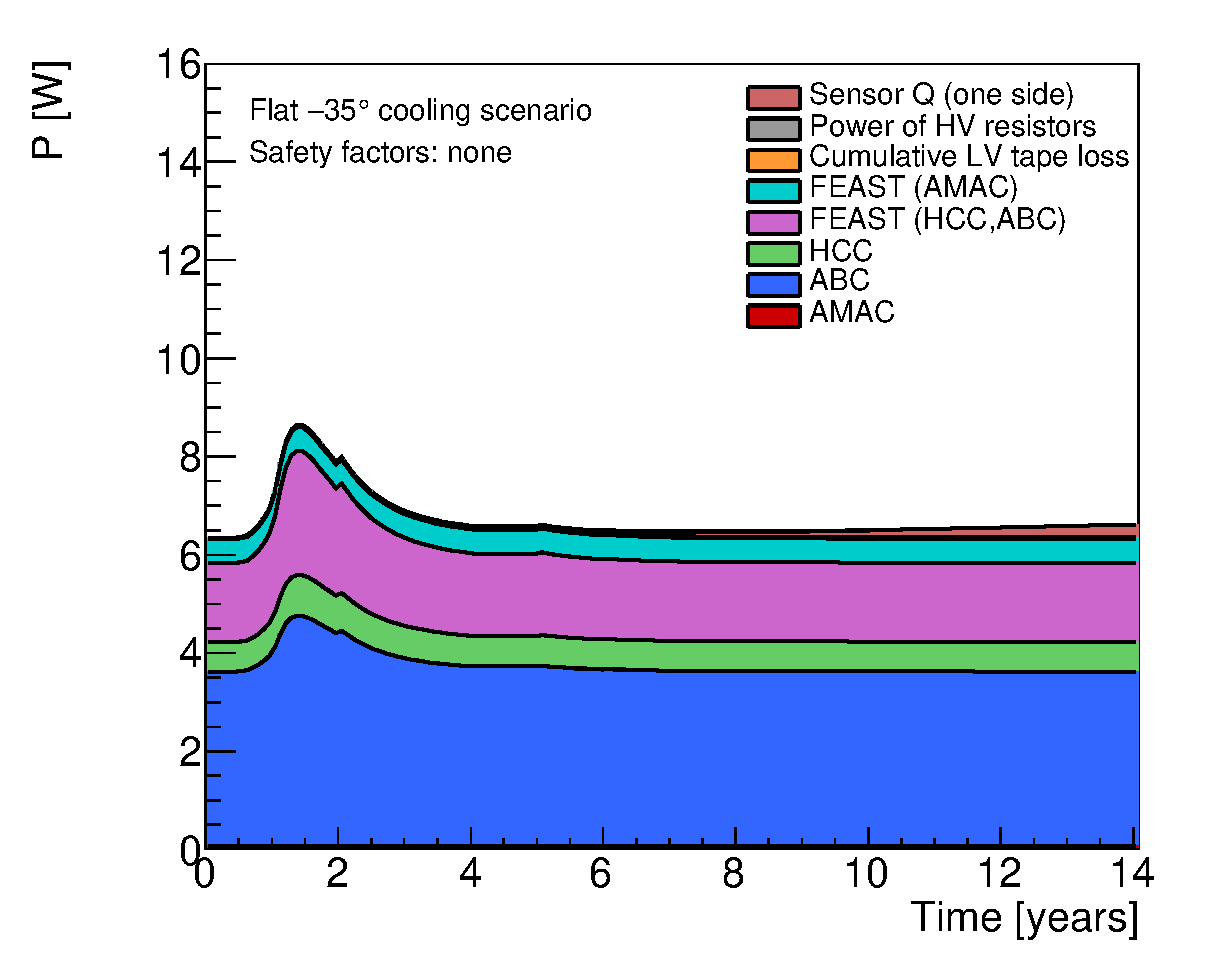
\includegraphics[width=0.59\linewidth]{figures/PowerStackPlot.eps}
\end{center}
\caption{Summary of the contributions of each front-end component to the total power in R1, given
a nominal TID bump parameterization and no safety factors, to illustrate the relative contributions
of each component.}
\label{power_stackplot}
\end{figure}

